\documentclass[12pt,spanish,letterpage, twoside, openright]{article}

\usepackage[labelfont=bf]{caption}
%\usepackage{fontspec}
\usepackage[T1]{fontenc}
\usepackage[utf8]{inputenc}
\usepackage[letterpaper]{geometry}
\geometry{verbose,tmargin=3cm,bmargin=3cm,lmargin=2.58cm,rmargin=2.58cm}
%\geometry{bindingoffset=0.80cm}%margen de impresion
\pagestyle{plain}
%\setlength{\parskip}{1ex plus 1mm minus 1mm}%espacio entre parrafos
\setlength{\parindent}{0.5cm}%tamaño de la sangrilla francesa
\usepackage{graphicx}
\usepackage{setspace}
\usepackage{tabulary}

\usepackage{babel}
\usepackage{multirow}
\providecommand{\tabularnewline}{\\}
\decimalpoint %punto decimal, en lugar de coma
\usepackage{array}
%\addto\shorthandsspanish{\spanishdeactivate{~<>}}
\date{}
\usepackage{multicol}
\usepackage[colorlinks=true, citecolor=blue, linkcolor=blue, urlcolor=blue]{hyperref}%colores para los hipervinculos
%para que no corte palabras
    \usepackage[none]{hyphenat}
\usepackage{amsmath}
\usepackage{amsfonts}
\usepackage{amssymb}
\usepackage{enumerate}
\usepackage{capt-of}
\usepackage[authoryear,bibnewpage]{natbib}

%\setlength{\columnseprule}{1pt}%linea entre columnas
\renewcommand{\baselinestretch}{1.5} % interlinado
\usepackage{capt-of}%%To get the caption fuera del entorno figure

%\usepackage[bibnewpage,natbibapa]{apacite}%bibliografia y citas en formato apa

\usepackage[load=prefixed, load=abbr]{siunitx}
\usepackage[arrowdel]{physics}

\newcommand{\diecte}{\mathbb{\epsilon}}
\newcommand{\h}{\text{h}}
\newcommand{\eV}{\text{eV}}%electron volts
\newcommand{\Hi}{\text{H}}%hidrogeno
\newcommand{\e}{\text{e}}%electron
\newcommand{\pow}[2]{\left( #1\right)^{#2} }
\newcommand{\Ms}{M_{\odot}}%simbolo de masa solar

%palabras frecuentes
\newcommand{\gtc}{Gran Telescopio Canarias~}
\newcommand{\gbt}{Green Bank Telescope~}
\newcommand{\object}{PSR J2042+0246~}


%para escribir codigo de otros lenguajes
\usepackage{listings}
%
\usepackage[dvipsnames]{xcolor}
\usepackage{soul}


\definecolor{codegreen}{rgb}{0,0.6,0}
\definecolor{codegray}{rgb}{0.5,0.5,0.5}
\definecolor{codepurple}{rgb}{0.58,0,0.82}
\definecolor{backcolour}{rgb}{0.95,0.95,0.92}

\lstdefinestyle{mystyle}{
	backgroundcolor=\color{backcolour},   
	commentstyle=\color{codegreen},
	keywordstyle=\color{magenta},
	numberstyle=\tiny\color{codegray},
	stringstyle=\color{codepurple},
	basicstyle=\ttfamily\footnotesize,
	breakatwhitespace=false,         
	breaklines=true,                 
	captionpos=b,                    
	keepspaces=true,                 
	numbers=left,                    
	numbersep=5pt,                  
	showspaces=false,                
	showstringspaces=false,
	showtabs=false,                  
	tabsize=1
}

\lstset{style=mystyle}



%--para generar apendice numerado
\usepackage{tocloft}
\usepackage[toc,page]{appendix}
\renewcommand{\appendixtocname}{ANEXOS}
\renewcommand{\appendixpagename}{ANEXOS}
\renewcommand{\appendixname}{Anexos}
%---para generar una tabla de anexos
\newcommand{\listanexoname}{{\Large Índice de anexos}}
\newlistof{anexo}{anx}{\listanexoname}
\newcommand{\anexo}[1]{%
	\refstepcounter{anexo}
	\par\noindent\textbf{{\large Anexo} \theanexo. #1}
	\addcontentsline{anx}{anexo}
	{\protect\numberline{\theanexo.}#1}\par}

\onehalfspacing
\begin{document}

	%\renewcommand{\BOthers}[1]{et al.\hbox{}}%esto cambia para multiples autores de "Cols" a "et al." respetando lo propuesto por normas apa.
	%\renewcommand{\BRetrievedFrom}{Recuperado de }%esto cambia la palabra "Descargado de" a "Recuperado de" respetando lo propuesto por normas apa.

%-----caratula
\begin{titlepage}
\setlength{\parindent}{0mm} %sangrilla de los parrafos
	\begin{center}
		
\includegraphics[scale=0.2]{img/LOGO-USAC-BNOFICIAL.pdf}\\
		{\huge \textbf{UNIVERSIDAD DE SAN CARLOS \vspace{5mm} \\ DE GUATEMALA}}\\
		~\\
		{\Large ESCUELA DE CIENCIAS FÍSICAS Y MATEMÁTICAS}\\
		{ \large LICENCIATURA EN FÍSICA APLICADA }\\
		~\\
		{\large ANTEPROYECTO DE TRABAJO PARA AÑO DE PRACTICAS}~\\
	\end{center}
	
	\begin{center}
		{\Large \textbf{ESTUDIO DEL SISTEMA BINARIO \linebreak PSR J2042+0246 \linebreak CON EL GRAN TELESCOPIO CANARIAS}
	\end{center}
	\vfill
	\begin{center}
		\textit{Elser Adolfo López Rosa}\\
		~\\~\\
		Dra. Aida Kirichenko\\ Asesora
		~\\~\\
		Dr. José Rodrigo Sacahuí Reyes\\ Supervisor
		~\\~\\
		Guatemala, 20 de enero de 2020
	\end{center}
\end{titlepage}



\setlength{\parindent}{0.5cm} %sangrilla de los parrafos

	
	
	
%%% Haga el diseño que más le guste
\chapter*{INTRODUCCIÓN}

Los objetos compactos son objetos exóticos, en ellos las teorías físicas se ponen a prueba, son los mejores laboratorios naturales en los que la materia se somete a condiciones extremas. Dentro los objetos compactos tenemos a las estrellas de neutrones, enanas blancas y agujeros negros. \\

Muchos de estos objetos exóticos podemos encontrarlos en sistemas binarios, uno de esos sistemas sumamente exótico son los denominados ``Black Widow'', estos sistemas están compuesto por una estrella de neutrones que gira rápidamente y emite radiación con la cual destruye o ``devora'' a su compa\~nera la cual típicamente es una estrella de secuencia principal. De este proceso típicamente destructivo es generalmente aceptado que los p\'ulsares de milisegundo aislados son pulsares que en su momento se encontraban en un sistema de este tipo.\\


Este proyecto se enfocar\'a en el análisis óptico utilizando datos obtenidos del telescopio óptico mas grande del mundo; El Gran Telescopio Canarias, en los filtros Sloan $g', r'$, e $i'$ y de ello obtener curvas de luz en cada uno de los filtros, as\'i como las gráficas de espectro de potencia. Por \'ultimo se deducirán parámetros  del sistema tales como:  la amplitud de la variación de la curva de luz en cada una de las bandas, el periodo orbital del sistema, la temperatura en la superficie del lado irradiado por el p\'ulsar (``day-side'') y el lado no irradiado (``night-side'') y la eficiencia calorífica de la estrella compa\~nera del p\'ulsar.







	
\input{obj-metodologia.tex}	
	
	
	
	
	
	\section{Descripción General de la Institución}
	%insitututo de investigacion de la USAC


La Universidad de San Carlos de Guatemala (USAC), es la única institución de educación superior de carácter público y autónomo con la que cuenta el país, fundada el 31 de enero de 1676 es esta la universidad más antigua de Centroamerica. Su sede principal se encuentra en la Ciudad Universitaria, Zona 12, de la Ciudad de Guatemala.\\

La Escuela de Ciencias Físicas y Matemáticas (ECFM), fundada en 2015 es la unidad académica que brinda actualmente las carreras de Física Aplicada y Matemática Aplicada en la Universidad de San Carlos. La ECFM cuenta con el Instituto de Investigación de Ciencias Físicas y Matemáticas (ICFM), que es la unidad que promueve y realiza investigación científica en los campos de Física y Matemática, los principales objetivos de trabajo del ICFM son:

\begin{itemize}
	\item Investigación académica en ciencia básica y aplicada
	\item Promoción de la investigación en ciencia básica y aplicada en el ámbito universitario
	\item  Difusión y divulgación de conocimiento generado por la investigación en ciencias físicas y matemáticas.
	\item  Actualización continua de programas académicos de ciencias físicas y matemáticas
\end{itemize}

\section{Objetivos}
\subsection{Objetivo General}
Caracterizar la compañera binaria del púlsar de milisegundo (MSP) \object utilizando los datos observacionales obtenidos con el  Gran Telescopio Canarias (GTC).
\subsubsection{Objetivos Específicos}
\begin{itemize}
    \item Realizar la reducción básica de datos utilizando IRAF y PyRAF.
    \item Localizar e identificar al objeto \object por medio de astrométria.
    \item Realizar la calibración fotométrica y calcular las magnitudes instrumentales en cada filtro.
    \item Determinar la temperatura efectiva, atmósfera, edad y masa de la estrella, utilizando los modelos de curvas de enfriamiento.
    \item Estimar la masa mínima del pulsar.
\end{itemize}


	\section{Descripción del Proyecto}


%{El objetivo del proyecto es}  caracterizar la compañera binaria del pulsar de milisegundo (MSP)   J2042+0246 utilizando los datos observacionales obtenidos con el  Gran Telescopio Canarias (GTC) {\color{OliveGreen}(Esto es el objetivo)}. \\



El proyecto consiste en analizar imágenes directas obtenidas con el telescopio óptico más grande del mundo\footnote{\url{http://www.gtc.iac.es/}} Gran Telescopio Canarias (GTC). En los filtros Sloan $g'$, $r'$ y $i'$ con el detector ``Optical System for Imaging and low-Intermediate-Resolution Integrated Spectroscopy'' (OSIRIS) que es un generador de imágenes y un espectrógrafo para el rango de longitud de onda óptica del GTC. Para ello se utilizará el Software ``Image Reduction and Analysis Facility'' (IRAF) y PYRAF que es un lenguaje de comandos para ejecutar tareas de IRAF
utilizando scripts de Python.
%descubierto por \citet{sanparsa}.  
\\ 

Primero se realizará la reducción básica de datos, es decir la sustracción de ``Bias'' o Imágenes Cero; éstas  permiten leer el nivel de ruido cero  en un CCD ya que son tomadas con tiempo cero de exposición, con ellas es posible determinar defectos de lectura que se aprecian como gradientes en la imagen  \citep[e.g.,][]{howell_2006,AvilaOAN}.
En un CCD  pueden existir variaciones en la sensibilidad de sus píxeles, es decir, no todos los píxeles tienen la misma respuesta a una fuente de iluminación. Para corregir este problema, se toman los llamados Campos Planos o ``Flat Fields''. Con los campos planos es posible corregir píxel a píxel las variaciones en el CCD, así como cualquier iluminación no uniforme en el CCD \citep[e.g.,][]{howell_2006,AvilaOAN}. Para éstas sustracciones se utilizará el método mostrado por \citet{AvilaOAN}. Luego se alinearán las imágenes de cada filtro para después ser combinadas y así aumentar el tiempo de exposición de cada filtro. \\

Posteriormente se realizará la referencia astrométrica con 20 estrellas del campo, no saturadas, del catalogo GAIA DR2 2018 \citep{gaia2}, para luego localizar el objeto utilizando las coordenadas medidas en radio, en un intervalo de confianza de $3\sigma'$ donde $\sigma'$ es la raiz del Error Cuadrático Medio (rms).   Después se realizará calibración fotométrica utilizando la estrella estándar SA 110-232 de \citet{smith2002} en cada filtro, para así obtener el ``Zero point'' o Punto Cero para con ello calibrar el sistema al sistema de magnitud estándar, ya que el flujo detectado de las estrellas variará de un detector a otro.\\

Para calcular la probabilidad de falsa identificación de la posición del objeto se utilizará la Distribución de Poisson $P=1-\exp(-\pi \sigma R^2)$ donde $\sigma$ y $R$ corresponden a la densidad numérica de las estrellas con magnitud similar y precisión astromética, respectivamente. \\

%{\color{OliveGreen}(Aquí hay que explicar como se encuentra el objeto de interés en las imágenes combinadas. También se puede 
%mencionar la probabilidad de la falsa identificación de la compañera óptica.)}

Por último utilizando Fotometría de Apertura, se determinarán las magnitudes \linebreak instrumentales del objeto en cada uno de los filtros. Luego se calculará la magnitud absoluta en el filtro $r'$ $(M_{r'}$), para que así utilizando diagramas de color-magnitud ($(r'-i')$ vs $M_{r'}$) y color-color ($(r'-i')$ vs $(g'-r')$)) con secuencias de enfriamiento de las enanas blancas \citep{holberg2006,kowalski2006, tremblay2011,bergeron2011}, con ello se determine si la compañera del sistema binario es una enana blanca. De ser así,  siguiendo el procedimiento descrito por \citet{dai2017} con ello pueda encontrarse la temperatura efectiva, atmósfera, edad y masa de la estrella. 





\section{Justificación del Proyecto}

Las enanas blancas y estrellas de neutrones son remanentes de estrellas que poseen características peculiares que surgen de someter la materia a condiciones extremas. Las enanas blancas poseen un  radio de $\sim$ 5000 km, densidades medias  de  $ \sim 10^6~ \g~ \cm^{-3}$, además su masa no puede ser mayor a $1.4 \Ms$ (éste valor es conocido como el limite de Chandrasekhar) \citep{lim-chandrasekhar,1983-shapiro}. Por otro lado las estrellas de neutrones si pueden exceder el limite de Chandrasekhar por lo que sus masas pueden encontrarse entre $1.0$-$2.14\Ms$ con densidades que incrementan con la profundidad, las cuales varían desde $\sim 10^6~\g~\cm^{-3}$ hasta $\sim \num{8e14}~\g~\cm^{-3}$. Las estrellas de neutrones poseen radios de $\sim 12~\km$ \citep{Camenzind2007,2011-rawls-mass-1Msolar,neutron-star-masss,2019-fonseca-mass214}. Uno de los mayores problemas  es el estado de los nucleones que la componen, ya que éstos pueden estar unidos en núcleos o estar libres en estados continuos \citep{Camenzind2007}. A las estrellas de neutrones que giran y emiten radiación de forma periódica se les denomina pulsar cuyos periodos de rotación van desde  $\sim 10^{-3}$ hasta  $\sim25$ segundos.\\


En el año 2013 el Telescopio Espacial de Rayos Gamma Fermi, con el \linebreak instrumento ``Large Area Telescope (LAT)'' que detecta fotones en el rango de $20 \mega \eV$ a 300 $\giga \eV$\footnote{\url{https://glast.sites.stanford.edu/}} recopiló una cantidad sustancial de datos que fue publicada en el catalogo 3FGL \citep{catalofermi2015}. En él 1010 objetos no fueron asociados con otras fuentes astrofísicas, por lo que  \citet{sanparsa} utilizando el radiotelescopio más importante del mundo\footnote{\url{https://greenbankobservatory.org/science/telescopes/gbt/}} de un solo disco (diámetro 100 metros)  \gbt (GBT) 
  para el proyecto de su tesis doctoral, utilizó estos datos para buscar fuentes asociadas en radio. Identificó así al objeto  \object como un sistema binario con un periodo de $77.2005806(3)$ días, que posee un MSP y otro objeto con limite inferior de masa de $0.18 \Ms $. \\


Por ultimo, las dos posibles distancias predichas por \citet{sanparsa} utilizando los modelos galácticos de densidad de electrones libres NE2001 \citep{NE2001} y YMW16 \citep{yao2017}, son menores a un kilparsec (1kpc), es decir NE2001  predice $0.83$ kpc y YMW16 predice $0.64$ kpc. Por esta razón debería ser posible observar la compañera en el rango óptico, sumado a ello las enanas blancas en general son difíciles de observar en otros rangos, tales como radio. Además con los resultados que se obtengan en el rango óptico también seria posible estimar la masa mínima del pulsar.  




   \section{Cronograma de Actividades} 

\begin{table}[h!]
\centering
\caption{Esquema del tiempo (en semanas), planificado para la realización de las actividades.}
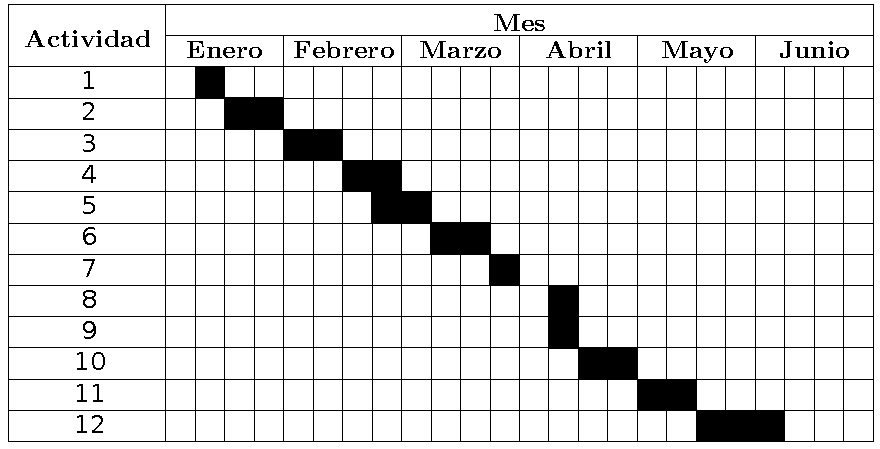
\includegraphics[scale=1]{img/crono.pdf}
\end{table}

\subsection{Descripción de las Actividades}
\begin{enumerate}
    \item Explorar diversas fuentes bibliográficas sobre objetos compactos, en particular sobre enanas blancas, estrellas de neutrones y púlsars.
    \item Explorar diversas fuentes bibliográficas sobre CCDs, Astro Fotometría y Astrométria.
    \item Estudiar la utilización de IRAF y PyRAF para la reducción y procesamiento de datos astronómicos.
    \item Realizar la reducción básica de las imágenes obtenidas del GTC.
    \item Alinear las imágenes obtenidas de la reducción y combinarlas, en cada filtro.
    \item Seleccionar un grupo de al menos 20 estrellas del campo, no saturadas para realizar la referencia astrométrica. Luego localizar el objeto.
    \item Realizar la calibración fotométrica y la probabilidad de obtener una falsa identificación.
    \item Determinar las magnitudes instrumentales del objeto en cada de los filtros.
    \item Calcular la magnitud absoluta en el filtro $r'$ y realizar los diagramas: color-magnitud y color-color.
    \item Determinar la temperatura efectiva, atmósfera, edad y masa de la estrella.
    \item Estimar la masa mínima del pulsar.
    \item Organizar y redactar el informe final de practicas.
    
\end{enumerate}


%ingreso de la bibliografía
\newpage
\setlength{\parskip}{0mm}
\spacing{1}
\bibliographystyle{mnras}
\bibliography{bibliografia}

\end{document} 



